\documentclass[paper=letter, fontsize=11pt]{scrartcl} % A4 paper and 11pt font size

\usepackage{float}
\usepackage[T1]{fontenc} % Use 8-bit encoding that has 256 glyphs
\usepackage{fourier} % Use the Adobe Utopia font for the document - comment this line to return to the LaTeX default
\usepackage[english]{babel} % English language/hyphenation
\usepackage{amsmath,amsfonts,amsthm} % Math packages
\usepackage{graphicx}
\usepackage{lipsum} % Used for inserting dummy 'Lorem ipsum' text into the template
\usepackage{hyperref}

\usepackage{sectsty} % Allows customizing section commands
\allsectionsfont{\centering \normalfont\scshape} % Make all sections centered, the default font and small caps

\usepackage{fancyhdr} 
\pagestyle{fancyplain} 
\fancyhead{} 
\fancyfoot[L]{}
\fancyfoot[C]{}
\fancyfoot[R]{\thepage} 
\renewcommand{\headrulewidth}{0pt}
\renewcommand{\footrulewidth}{0pt} 
\setlength{\headheight}{13.6pt} 

\numberwithin{equation}{section} 
\numberwithin{figure}{section} 
\numberwithin{table}{section} 

\setlength\parindent{0pt} 

%----------------------------------------------------------------------------------------
%	TITLE SECTION
%----------------------------------------------------------------------------------------

\newcommand{\horrule}[1]{\rule{\linewidth}{#1}}

\title{	
\normalfont \normalsize 
\textsc{University of California Irvine} 
\textsc{Course: Organization of Digital Computers Laboratory (112L) \\ Winter 2016} \\ [25pt]
\horrule{0.5pt} \\[0.4cm] % Thin top horizontal rule
\huge Lab 2 Report - Single-Cycle MIPS Datapath and Control\\
\horrule{2pt} \\[0.5cm] % Thick bottom horizontal rule
}
\author{Prepared by: Team The Powerful Processors \\ Jon Raphael Apostol - 32302252 \\ Binh Nguyen - 34707912 \\ Yixiang Yan - 16392389 \\ James Yi - 17492099 } % Your name


\date{\normalsize\today} % Today's date or a custom date

\begin{document}

\maketitle % Print the title

%----------------------------------------------------------------------------------------
%	INTRODUCTION
%----------------------------------------------------------------------------------------

\section{Introduction}
In this lab, we implemented the single-cycle MIPS processor in VHDL. Since it is a single-cycle processor, there are no branch instructions, and the ALU only does addition, subtraction, the AND operation, the OR operation, the XOR operation, and the NOR operation. The branch instruction will be implemented in the later labs.

\pagebreak

%----------------------------------------------------------------------------------------
%	DESIGN
%----------------------------------------------------------------------------------------

\section{Design}
\begin{center}
For our processor, we designed it in the following different blocks:
\end{center}
\begin{itemize}
	\item The Program Counter (PC)
	\begin{enumerate}
		\item The program counter contains the address of the instruction that is being executed.
		\item For our program counter we add 1 to the address everytime the clock hits a rising edge.
	\end{enumerate}
	\item The Instruction Memory (ROM)
	\begin{enumerate}
		\item The instruction memory is implemented as a ROM. This is where the processor will receive the instructions from.
		\item The imem.h file is where we store instructions in hexadecimal form. 
	\end{enumerate}
	\item The Register File
	\begin{enumerate}
		\item The register file contains all the registers that each may store 32-bits of data.
	\end{enumerate}
	\item The Data Memory (RAM)
	\begin{enumerate}
		\item The data memory will be a 512 long array of words with 32-bits each word.
	\end{enumerate}
	\item The ALU
	\begin{enumerate}
		\item The ALU is where the mathematics of the processor is carried out and then stored in either the register file or the data memory.
	\end{enumerate}
	\item The Sign Extender
	\begin{enumerate}
		\item The sign extender lengthens the 15 downto 0 bits of the instruction to 32-bits as a way to carry out I-type instructions.
	\end{enumerate}
	\item The Multiplexer
	\begin{enumerate}
		\item The multiplexer selects one of two choices. This is used throughout the processor to select the type of instruction.
	\end{enumerate}
	\item The Controller
	\begin{enumerate}
		\item The controller chooses the ALU control and is also a factor in controlling the type of instruction.
	\end{enumerate}
	\item The ALU Control
		\begin{enumerate}
		\item Currently this is not being implemented, but it a way to increase the speed of the processor.
		\item This selects the operation the ALU will be doing.
	\end{enumerate}
\end{itemize}

\pagebreak

%----------------------------------------------------------------------------------------
%	TESTBENCH
%----------------------------------------------------------------------------------------

\section{Tests}
\begin{center}
These are the tests we did on multiple commands that were given. We initialized the \$1 to be equal to 1 in our code to test these instructions. Each instruction below was done in order.
\end{center}
Store Word (SW):

\begin{figure}[H]
	\centering
		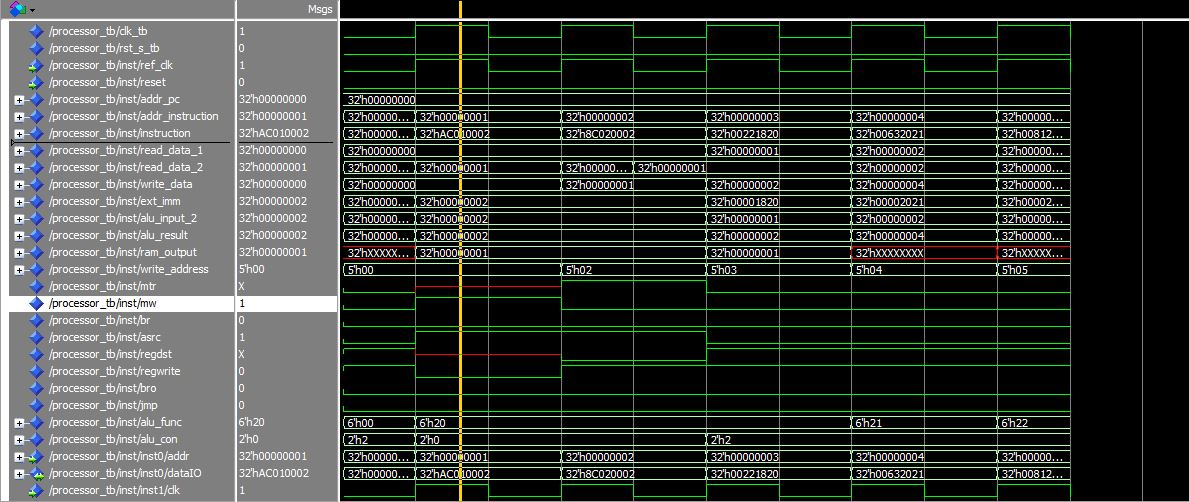
\includegraphics[width=150mm]{../sim/photo/sw.JPG}
	\label{fig:sw}
\end{figure}

Hexadecimal:
ac010002
\\
\\
Binary:
\\
101011 00000 00001 0000000000000010
\\
\\
MIPS Code:
\\
sw \$0, \$0, \$1
\\
\\
This instruction stores the word from register 1 to register 0, thus making register 0 equal to '1';
\\
\pagebreak
\\
Load Word (LW):

\begin{figure}[H]
	\centering
		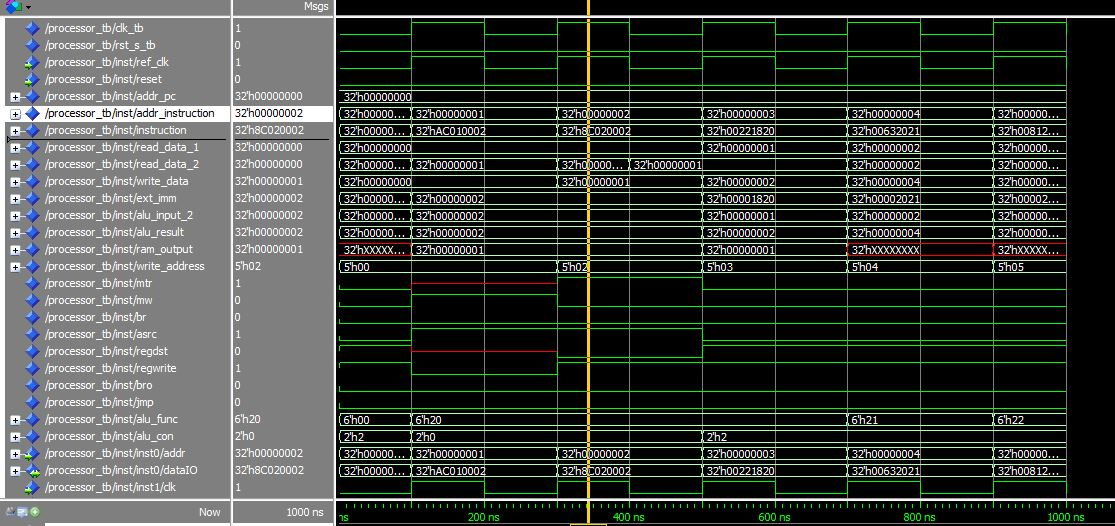
\includegraphics[width=150mm]{../sim/photo/lw.JPG}
	\label{fig:lw}
\end{figure}

Hexadecimal:
\\
8c020002
\\
\\
Binary:
\\
100011 00000 00010 0000000000000010
\\
\\
MIPS Code:
\\
lw \$2, \$0,  \$2
\\
\\
This instruction loads the word from register 0 into register 2, thus making register 2 equal to '1'.
\\
\pagebreak
\\
ADD:

\begin{figure}[H]
	\centering
		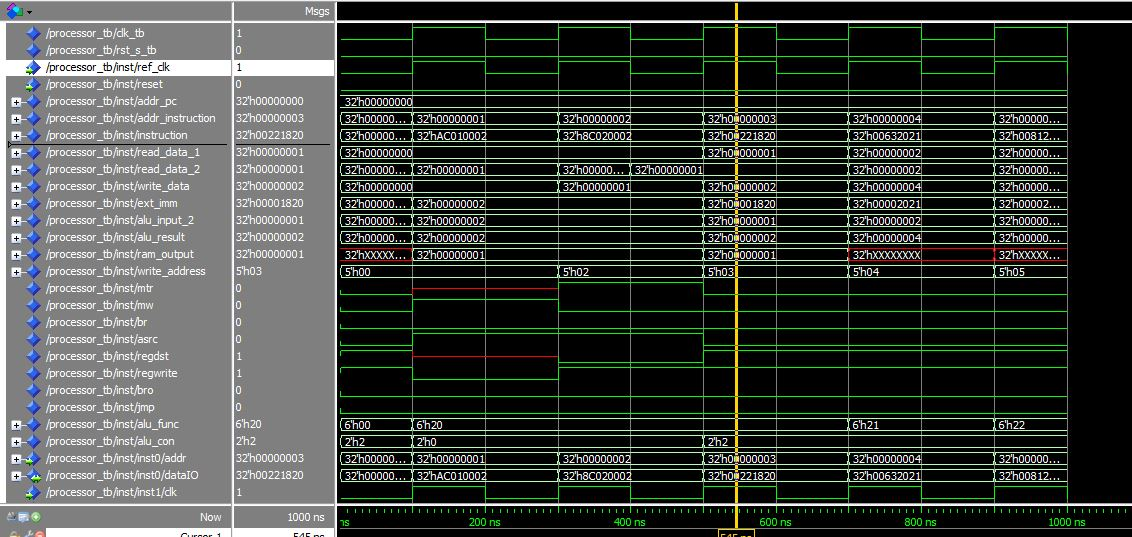
\includegraphics[width=150mm]{../sim/photo/add.JPG}
	\label{fig:ADD}
\end{figure}

Hexadecimal:
\\
00221820
\\
\\
Binary:
\\
000000 00001 00010 00011 00000 100000
\\
\\
MIPS Code:
\\
add \$3, \$1, \$2
\\
\\
This instruction adds register 1 with register 2 and then stores the value in register 3, thus making register 3 equal to '2'.
\\
\\
\\
Hexadecimal:
\\
00632021 
\\
\\
Binary:
\\
000000 00011 00011 00100 00000 100001
\\
\\
MIPS Code:
\\
add \$4, \$3, \$3
\\
\\
This instruction adds register 3 with register 3 and then stores the value in register 4, thus making register 4 equal to '4'.
\pagebreak
\\
SUB:

\begin{figure}[H]
	\centering
		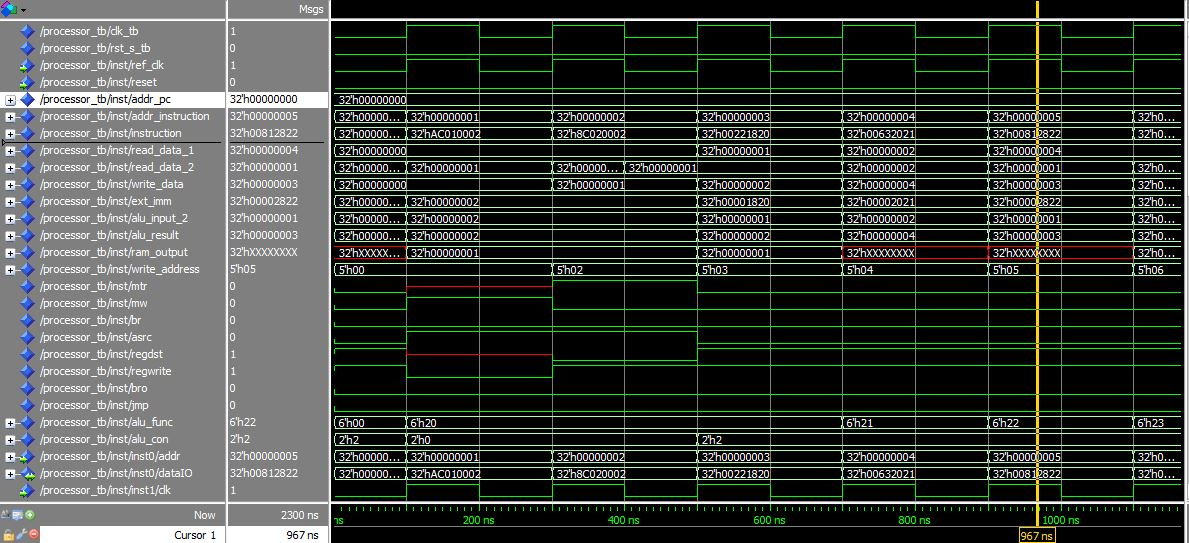
\includegraphics[width=150mm]{../sim/photo/sub.JPG}
	\label{fig:SUB}
\end{figure}

Hexadecimal:
\\
00812822
\\
\\
Binary:
\\
000000 00100 00001 00101 00000 100010
\\
\\
MIPS Code:
\\
sub \$5, \$4, \$1
\\
\\
This instruction subtracts the value of register 1 from the value of register 4 then stores the value into register 5, thus making register 5 equal to '3'.
\\
\\
\\
Hexadecimal:
\\
00833023
\\
\\
Binary:
\\
000000 00100 00011 00110 00000 100011
\\
\\
MIPS Code:
\\
sub \$6, \$4, \$3
\\
\\
This instruction subtracts the value of register 3 from the value of register 4 then stores the value into register 6, thus making register 6 equal to '2'.
\pagebreak
\\
AND:

\begin{figure}[H]
	\centering
		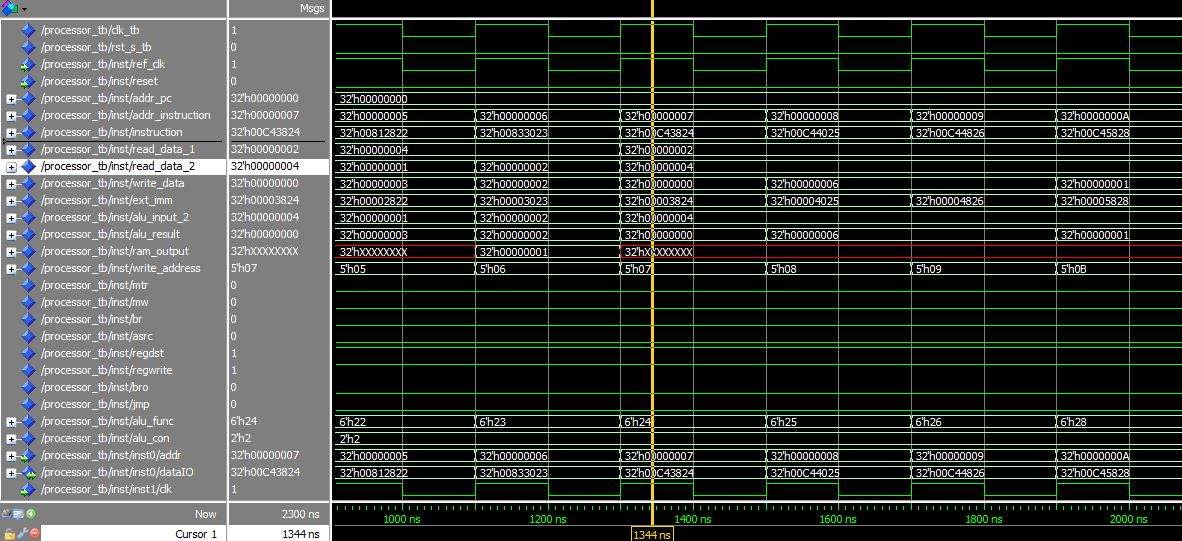
\includegraphics[width=150mm]{../sim/photo/and.JPG}
	\label{fig:AND}
\end{figure}

Hexadecimal:
\\
00c43824
\\
\\
Binary:
\\
000000 00110 00100 00111 00000 100100
\\
\\
MIPS Code:
\\
and \$7, \$6, \$4
\\
\\
This instruction takes the bitwise AND of register 6 and register 4 then stores the value into register 7, thus making register 7 equal to '0'.
\\
\pagebreak
\\
OR:

\begin{figure}[H]
	\centering
		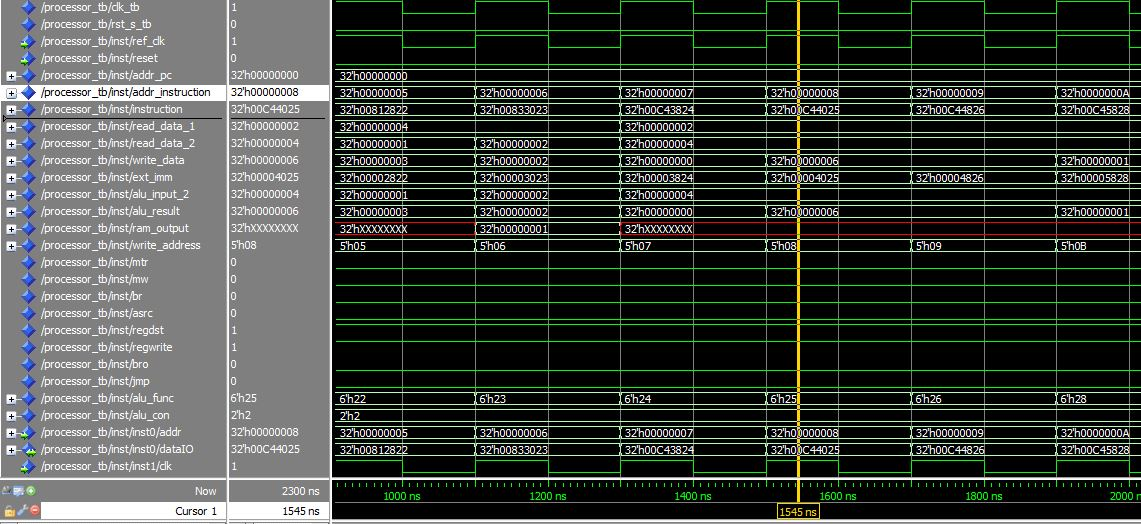
\includegraphics[width=150mm]{../sim/photo/or.JPG}
	\label{fig:OR}
\end{figure}

Hexadecimal:
\\
00c44025
\\
\\
Binary:
\\
000000 00110 00100 01000 00000 100101
\\
\\
MIPS Code:
\\
or  \$8, \$6, \$4
\\
\\
This instruction takes the bitwise OR of register 6 and register 4 then stores the value into register 8, thus making register 8 equal to '6'.
\\
\pagebreak
\\
XOR:

\begin{figure}[H]
	\centering
		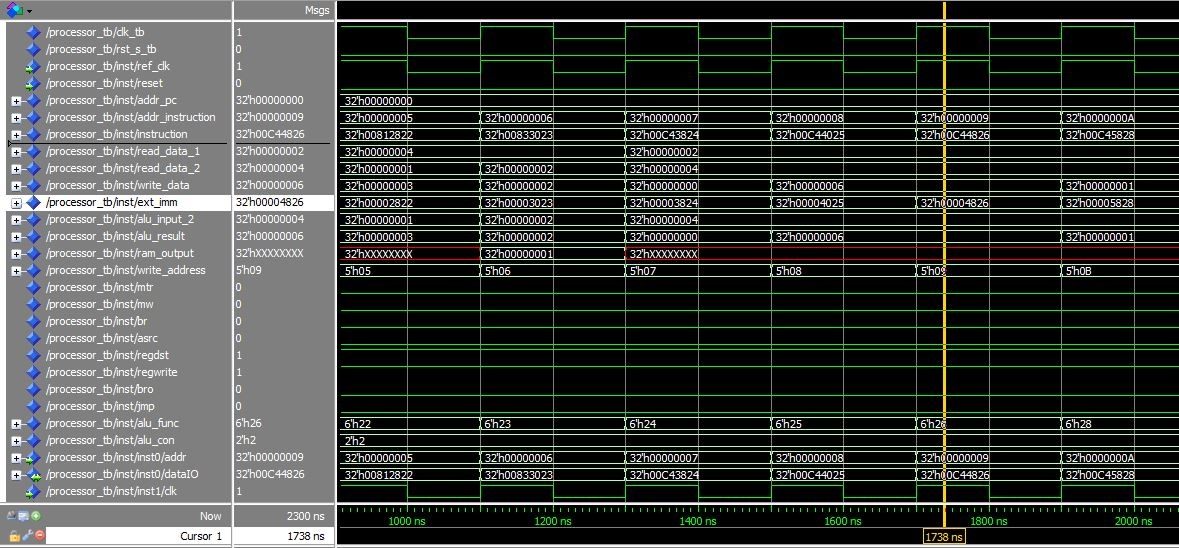
\includegraphics[width=150mm]{../sim/photo/xor.JPG}
	\label{fig:XOR}
\end{figure}

Hexadecimal:
\\
00c44826
\\
\\
Binary:
\\
000000 00110 00100 01001 00000 100110
\\
\\
MIPS Code:
\\
xor \$9, \$6, \$4
\\
\\
This instruction takes the bitwise XOR of register 6 and register 4 then stores the value into register 9, thus making register 9 equal to '6'.
\\
\pagebreak
\\
Set-Less-Than Signed: 

\begin{figure}[H]
	\centering
		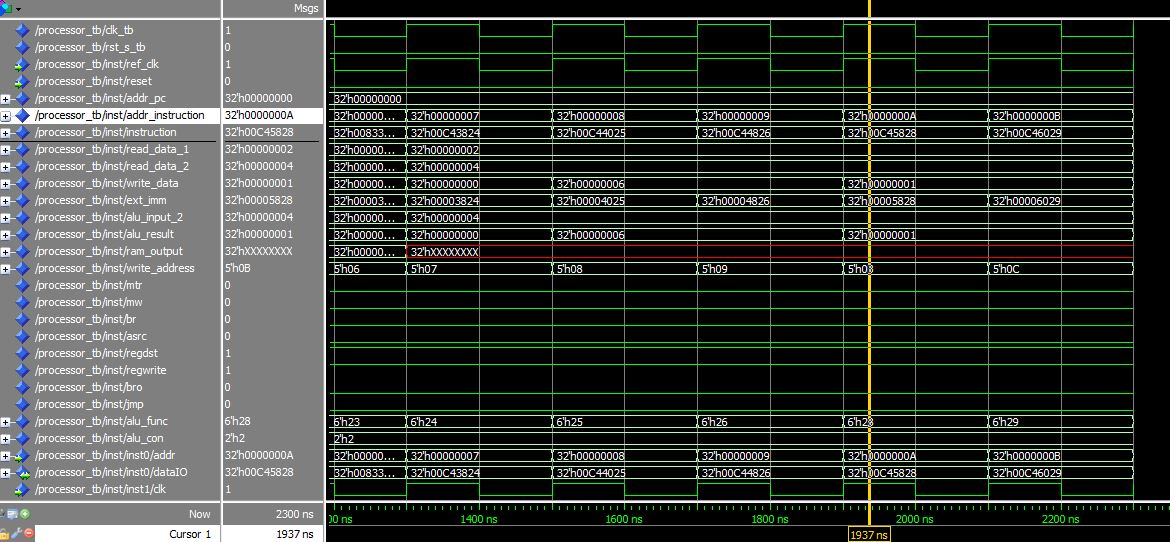
\includegraphics[width=150mm]{../sim/photo/setlessthansigned.JPG}
	\label{fig:Set-Less-Than Signed}
\end{figure}

Hexadecimal:
\\
00c45828
\\
\\
Binary:
\\
000000 00110 00100 01011 00000 101000
\\
\\
MIPS Code:
\\
slt \$6, \$4, \$11 (2<4 \$11=1)
\\
\\
This instruction checks whether or not the signed value register 6 is less than the signed value register 4 then stores '0' (false) or '1' (true) into register 11, thus making register 11 equal to '1'.
\\
\pagebreak
\\
Set-Less-Than Unsigned:

\begin{figure}[H]
	\centering
		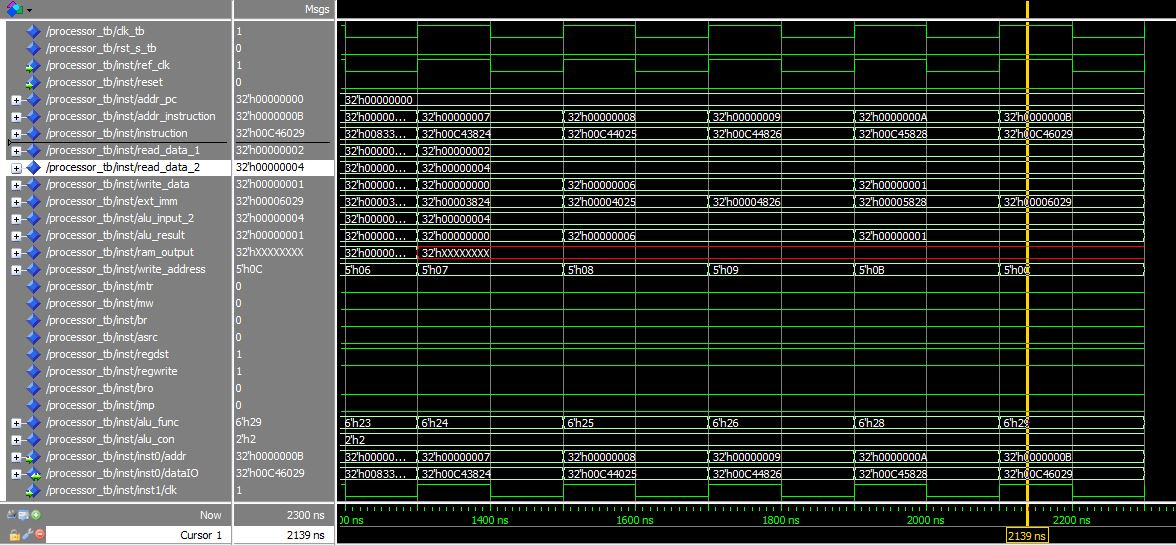
\includegraphics[width=150mm]{../sim/photo/setlessthanunsigned.JPG}
	\label{fig:Set-Less-Than Unsigned}
\end{figure}

Hexadecimal:
\\
00c46029
\\
\\
Binary:
000000 00110 00100 01100 00000 101001
\\
\\
MIPS Code:
\\
slt(unsigned) \$12, \$6, \$4
\\
\\
This instruction checks whether or not the unsigned value of register 6 is less than unsigned value of register 4 then stores '0' (false) or '1' (true) into register 12, thus making register 12 equal to '1'.
\\
\pagebreak
\\
NOR:

\begin{figure}[H]
	\centering
		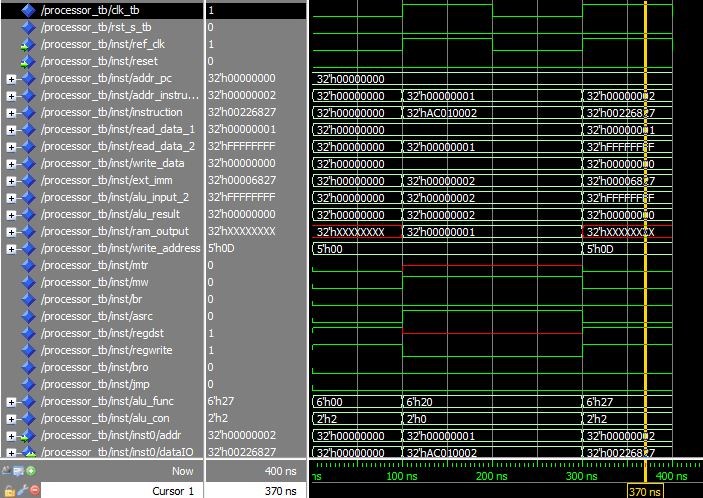
\includegraphics[width=150mm]{../sim/photo/nor.JPG}
	\label{fig: NOR}
\end{figure}

For the NOR instruction we set register 1 to '1' and register 2 to '11111111'.
\\
\\
Hexadecimal:
\\
00226827
\\
\\
Binary:
\\
000000 00001 00010 01101 00000 100111
\\
\\
MIPS Code:
\\
nor \$13, \$1, \$2
\\
\\
This instruction takes the bitwise NOR of register 1 and register 2 then stores the value into register 13, thus making register 13 equal to '0'.
\\
\pagebreak
\\
RESET:

\begin{figure}[H]
	\centering
		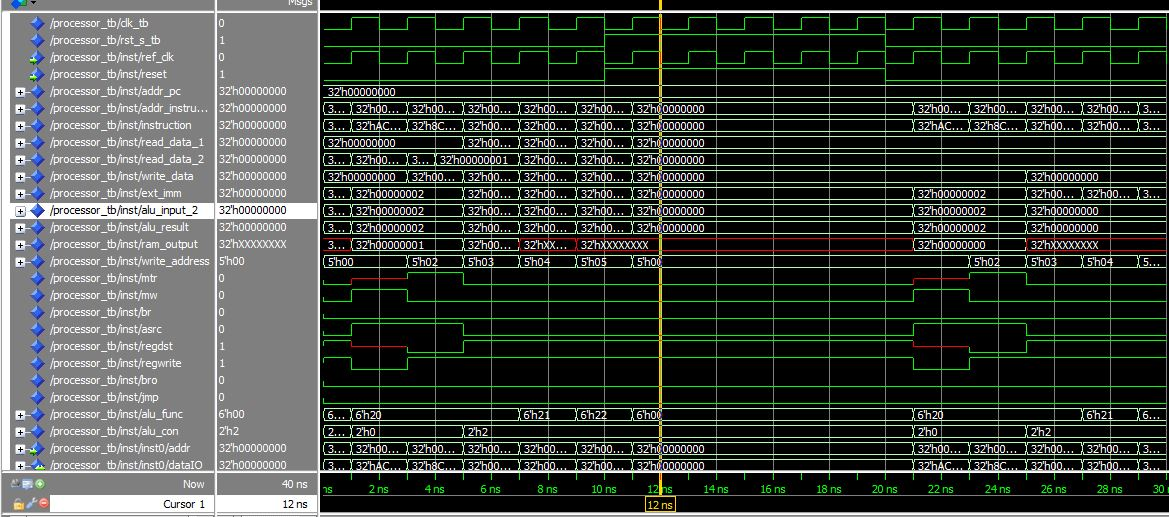
\includegraphics[width=150mm]{../sim/photo/reset.JPG}
	\label{fig:Reset}
\end{figure}

The reset after 10 ns


%----------------------------------------------------------------------------------------
%	CONCLUSION
%----------------------------------------------------------------------------------------

\section{Conclusion}
In the end, our program compiled fully with some warnings here and there. We also ended up having a run time of less than 1 ns per instruction.



\end{document}